% !TEX root = ../ac_paper.tex

\section{Introduction\label{sec:intro}}


\begin{figure}
	\centering
	\begin{subfigure}[b]{0.5\textwidth}
		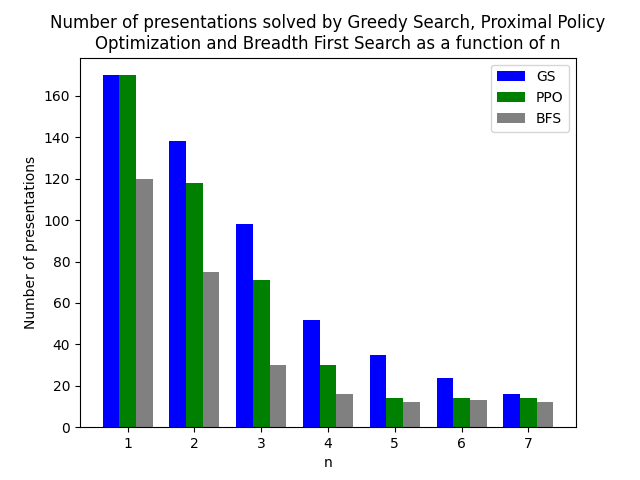
\includegraphics[width=1.1\textwidth]{fig/performance_vs_n.png}
		\caption{Distribution versus $n$}
		\label{fig:performance_vs_n}
	\end{subfigure}
	
	\begin{subfigure}[b]{0.5\textwidth}
		\centering
		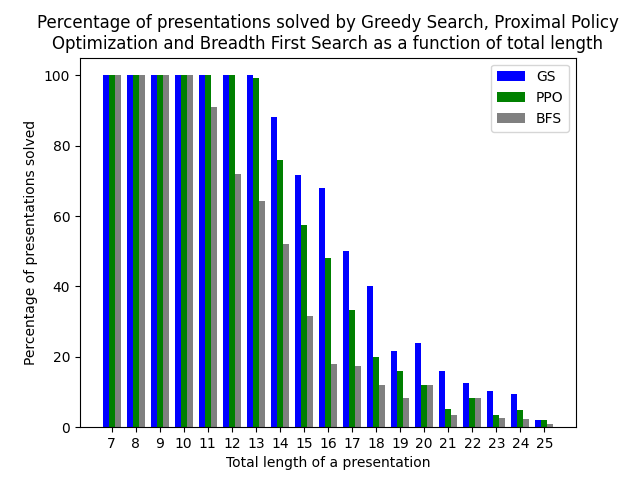
\includegraphics[width=1.1\textwidth]{fig/performance_vs_length.png}
		\caption{Distribution versus total length}
		\label{fig:performance_vs_length}
	\end{subfigure}
	\caption{The figure shows the number of presentations from the Miller-Schupp series that were solved using Greedy Search (GS) and Breadth-First Search (BFS) as a function of \( n \). Greedy Search consistently outperforms Breadth-First Search. Specifically, Greedy Search successfully solved all 170 presentations of the Miller-Schupp series with \( n=1 \) in our dataset.} \label{fig:performance}
	
\end{figure}

Figure \autoref{fig:performance} compares the performance of Greedy Search (GS), Breadth First Search and Proximal Policy Optimization on the presentations of Miller-Schupp series with $n, \ \text{length}(w) \leq 7$.
